%%% Copyright (C) 2017 Vincent Goulet
%%%
%%% Ce fichier fait partie du projet «Programmer avec R»
%%% http://github.com/vigou3/programmer-avec-r
%%%
%%% Cette création est mise à disposition selon le contrat
%%% Attribution-Partage dans les mêmes conditions 4.0
%%% International de Creative Commons.
%%% http://creativecommons.org/licenses/by-sa/4.0/

\chapter{Éléments d'informatique pour programmeurs}
\label{chap:informatique}

% Intro du chapitre

\section{Bref historique des langages de programmation}
\label{sec:informatique:historique}

Ada Lovelace (1815--1852) est généralement reconnue comme la première
auteure d'un algorithme et de ce que l'on appelle aujourd'hui un
programme informatique. C'est en son honneur qu'été nommé le langage
Ada conçu en réponse à un cahier de charges du département de la
Défense des États-Unis au début des années 1980.

Franchissons d'un bond les premiers jours de l'informatique et de la
programmation pour arriver aux ordinateurs électriques modernes, dans
les années 1940. On programme alors généralement ceux-ci en
\emph{assembleur}, un langage de très bas niveau facilement
interprétable par la machine, mais difficile à lire par des humains,
comme l'extrait de programme de la
\autoref{fig:informatique:assembleur} le démontre bien.

\begin{figure}
  \centering
  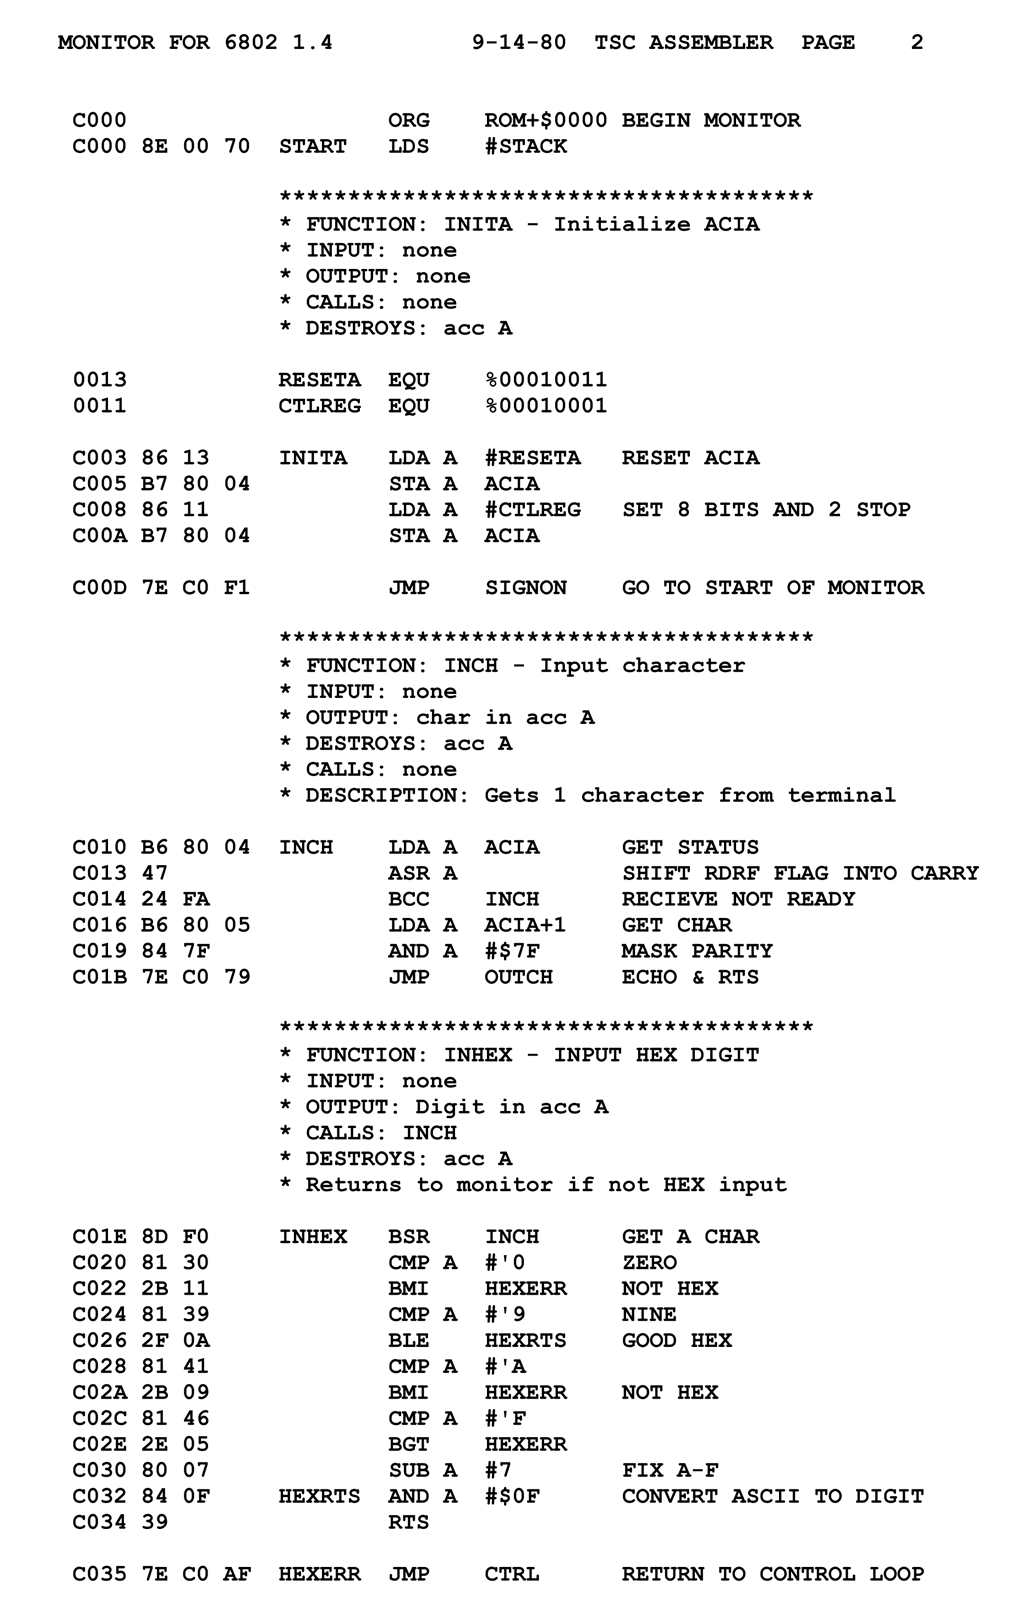
\includegraphics[trim=0 475 0 0, clip=true]{Motorola_6800_Assembly_Language.png}
  \caption[Programme en assembleur pour un microprocesseur 8~bits
  Motorola 6800.]{Extrait d'un programme en assembleur pour un
    microprocesseur 8~bits Motorola 6800. {\small Source:
      \link{https://commons.wikimedia.org/wiki/File\%3AMotorola_6800_Assembly_Language.png}{Wikimedia
        Commons}}}
  \label{fig:informatique:assembleur}
\end{figure}

Les premiers langages créés pour transmettre des instructions à un
ordinateur apparaissent dans les années 1950. Ils sont à l'origine
intimement liés à l'architecture d'un ordinateur: à chaque type
d'ordinateur son langage de programmation. Certaines contraintes ---
ou exigences --- des langages de l'époque proviennent aussi du support
physique alors utilisé pour stocker les programmes: les cartes
perforées.

\subsection{Fortran}
\label{sec:informatique:historique:fortran}

En 1954, l'ingénieur de IBM John Backus publie les spécifications du
langage FORTRAN (\emph{FORmula TRANslating System}). Le premier
compilateur voit le jour deux ans plus tard. Fortran (avec des
minuscules à partir de 1977) deviendra rapidement le langage standard
dans le calcul scientifique.

Plus d'un demi-siècle plus tard, l'empreinte de Fortran demeure
importante, notamment grâce aux bibliothèques d'algèbre linéaire
BLAS\footnote{%
  \emph{Basic Linear Algebra Subprograms};
  \link{http://www.netlib.org/blas}{}.} %
et LAPACK\footnote{%
  \emph{Linear Algebra PACKage};
  \link{http://www.netlib.org/lapack}{}.} %
auxquelles ont recours la plupart des progiciels scientifiques, dont
R. Le langage est toujours utilisé en calcul haute performance et pour
mesurer le rendement des superordinateurs.

\begin{figure}[t]
  \notebox{Dans le très recommandable film Les figures de l'ombre
    (\emph{Hidden Figures}, 2016), une des héroïnes entreprend de
    s'attaquer à la programmation des nouveaux ordinateurs de la NASA.
    On peut alors voir qu'elle apprend le Fortran.}
\end{figure}

\subsection{Lisp}
\label{sec:informatique:historique:lisp}

Le deuxième langage le plus ancien toujours largement diffusé est Lisp
(\emph{LISt Processing}). Créé par John McCarthy en 1958 en tant que
modèle pratique pour représenter des programmes, le Lisp est devenu le
langage de choix pour la recherche et les applications en intelligence
artificielle. Le terme Lisp désigne aujourd'hui une famille de
langages comprenant de nombreux dialectes, dont Common Lisp, Scheme et
Emacs Lisp.

Le Lisp se distingue en outre par une syntaxe simple en notation
préfixée (voir encadré), le support pour la programmation
fonctionnelle (\autoref{sec:informatique:paradigmes}) et la faculté de
manipuler le code source en tant que structure de données. Autre trait
distinctif: la syntaxe du Lisp fait un usage immodéré des parenthèses.

Le Lisp est entouré d'une aura de beauté et d'élégance dont peu
d'autres langages peuvent se targuer. Citons Eric Raymond dans
\link{http://www.catb.org/esr/faqs/hacker-howto.html}{\emph{How to
    Become a Hacker}}:
\begin{quote}
  Il faut apprendre le Lisp pour l'extraordinaire expérience d'éveil
  [\emph{enlightenment experience}] que procure le fait de finalement
  le comprendre; cette expérience fera de vous un meilleur programmeur
  pour toujours, même si vous n'avez plus vraiment à utiliser le Lisp.
\end{quote}

Pour illustrer encore davantage la place toute particulière qu'occupe
le Lisp en programmation, mentionnons également l'aphorisme selon
lequel «ceux qui ne connaissent pas le Lisp sont condamnés à le
réinventer», d'une certaine façon la version courte de la célèbre
\link{https://en.wikipedia.org/wiki/Greenspun\%27s_tenth_rule}{\emph{Greenspun's
    tenth rule of programming}}: %
\begin{quote}
  Tout programme en C ou en Fortran suffisamment complexe contient une
  implémentation mal spécifiée, pleine de bogues et lente de la moitié
  de Common Lisp.
\end{quote}
(Fait amusant à noter: il n'y a pas d'autres lois que la dixième, de
l'\link{http://philip.greenspun.com/bboard/q-and-a-fetch-msg?msg_id=000tgU}{aveu
  même de l'auteur}.)

\begin{figure}[t]
  \label{fig:informatique:notations}
  \setlength{\FrameRule}{1pt}
  \lstset{backgroundcolor=\color{codebg},
    frame=lr, rulecolor=\color{codebg},
    xleftmargin=3.4pt, xrightmargin=3.4pt}
  \begin{emphbox}{\mdseries Notations infixée, préfixée et suffixée}
    Les notations infixée (\emph{infix}), préfixée (\emph{prefix}) et
    suffixée (\emph{postfix}) sont trois manières différentes, mais
    équivalentes, d'écrire des expressions en mathématiques ou en
    programmation.

    Par exemple, l'opération d'addition de deux opérandes $x$ et $y$
    s'écrit en notation infixée
\begin{lstlisting}
x + y
\end{lstlisting}
    En notation préfixée, aussi appelée notation polonaise,
    l'opérateur est placé \emph{avant} les opérandes:
\begin{lstlisting}
+ x y
\end{lstlisting}
    On l'aura compris, en notation suffixée, ou notation polonaise
    inversée, l'opérateur apparait \emph{après} les opérandes:
\begin{lstlisting}
x y +
\end{lstlisting}
    Nous sommes davantage habitués à lire la notation infixée, quoique
    la notation préfixée nous soit familière pour les opérateurs à un
    seul opérande (comme la négation) ou pour les appels de fonctions.
    La notation suffixée n'a jamais recours aux parenthèses.

    La compagnie HP commercialise de très prisées calculatrices
    scientifiques utilisant la notation suffixée (libellées RPN pour
    \emph{Reverse Polish Notation}) depuis 1972.
  \end{emphbox}
\end{figure}

\subsection{COBOL}
\label{sec:informatique:historique:cobol}

Le troisième langage développé dans les années 1950 et toujours en
usage de nos jours est COBOL (\emph{COmmon Business Oriented
  Language}). Ce langage spécialisé dans les applications de gestion a
été créé en 1959 par un comité formé pour proposer un langage commun
pour l'administration américaine.

Le COBOL reste très utilisé dans de grandes entreprises, notamment
dans les institutions financières. La légende urbaine veut d'ailleurs
que les programmeurs COBOL soient comparativement très bien rémunérés
aujourd'hui sous l'effet combiné de leur rareté et de l'importance
opérationnelle des applications qu'ils doivent maintenir.

\subsection{Algol}
\label{sec:informatique:historique:algol}

Dès la fin de la décennie 1950, un comité de scientifiques se réunit à
Zurich pour concevoir ce que l'on voudrait voir devenir le langage de
programmation standard. De ces rencontres naîtra Algol
(\emph{ALGorithmic Oriented Language}) en 1958. Comme la plupart des
tentatives de définition d'un standard, c'est un échec: le langage est
populaire dans les milieux académiques, mais restera peu utilisé dans
les applications commerciales.

Cela dit, on doit à Algol plusieurs innovations importantes, de telle
sorte qu'un grand nombre des langages qui verront le jour par la suite
seront considérés comme ses descendants; le poster
\link{http://www.oreilly.com/go/languageposter}{\emph{History of
    Programming Languages}} de O'Reilly Media illustre ce fait à
merveille. \citet{Hoare:1973} a d'ailleurs cette jolie formule:
\begin{quote}
  Voici un langage très en avance sur son temps, il n'a pas seulement
  été une amélioration de ses prédécesseurs mais aussi une
  amélioration de presque tous ses successeurs.
\end{quote}


\begin{figure}[t]
  \centering
  \begin{minipage}{0.9\linewidth}
    \setkeys{Gin}{width=\textwidth}
    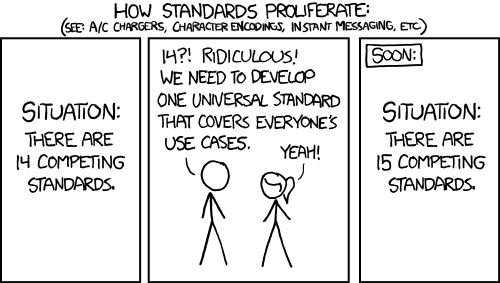
\includegraphics{standards} \\
    \footnotesize\sffamily%
    Tiré de \href{http://xkcd.com/927/}{XKCD.com}
  \end{minipage}
\end{figure}

\subsection{APL}
\label{sec:informatique:historique:apl}

Notre historique ne serait pas complet sans un mot sur APL (\emph{A
  Programming Language}, qui l'aurait cru). Même s'il n'a jamais connu
une diffusion importante, ce langage conçu par Kenneth Iverson autour
de 1962 n'en a pas moins eu une influence considérable sur la manière
de penser et de représenter les opérations mathématiques sur les
tableaux à plusieurs dimensions.

Doté d'une large gamme de symboles pour représenter des opérations et
d'une syntaxe tout à fait particulière --- les expressions sont
exécutées de droite à gauche! --- l'APL est remarquablement concis et
puissant; voir la \autoref{fig:informatique:apl} pour un aperçu. Le
revers de la cette médaille et ce qui a assurément nui à son adoption
à large échelle, c'est la difficulté que l'on éprouve à relire le
code. Assez pour que d'aucuns qualifient l'APL de «langage à écriture
seulement».

APL a pendant longtemps été un langage très prisé par les actuaires,
aussi subsiste-t-il du code dans certaines compagnies d'assurance. Le
modèle de traitement des vecteurs, matrices et tableaux de l'APL a
servi d'inspiration pour la conception du langage S --- nous y
reviendrons au \autoref{chap:presentation}.

Le langage continue sa vie aujourd'hui principalemnt sous forme de son
successeur, J.

\begin{figure}
  \centering
  \scalebox{0.4}{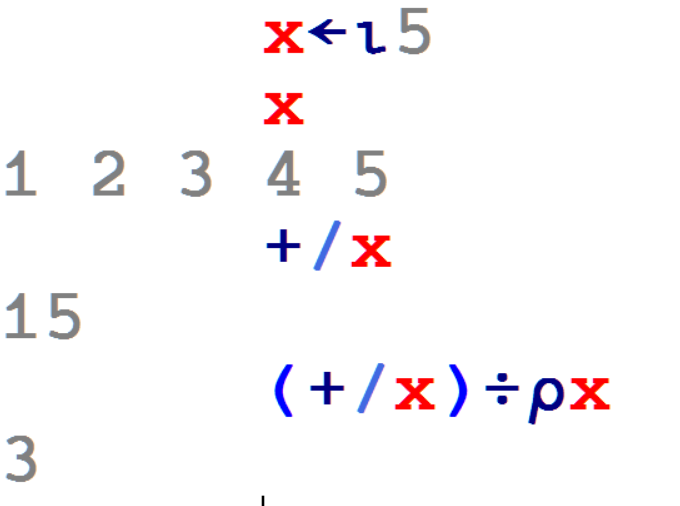
\includegraphics{APL_intro}}
  \caption[Opérations simples en APL.]{Opérations simples en APL. De
    haut en bas: génération des nombres de $1$ à $5$ et stockage dans
    la variable \code{x}; affichage du contenu de \code{x}; somme des
    éléments de \code{x}; moyenne des éléments de \code{x}. {\small Source:
    François-Dominique,
    \link{https://commons.wikimedia.org/w/index.php?curid=43207460}{Wikimedia
      Commons}, CC BY-SA 4.0}}
  \label{fig:informatique:apl}
\end{figure}

\subsection{C}
\label{sec:informatique:historique:c}

Le langage C a été inventé en 1972 chez Bell Labs par Ken Thompson et
Dennis Ritchie afin de réécrire le système d'exploitation UNIX
(\autoref{sec:informatique:os:unix}). Il demeure beaucoup utilisé pour
la programmation système: le noyau de systèmes d'exploitation comme
Windows et Linux sont développés en grande partie en C.

Le C est un langage de programmation généraliste considéré, selon les
standards actuels, comme de bas niveau. Pour illustrer, l'utilisateur
doit programmer des traitements comme la libération de la mémoire, la
vérification de la validité des indices sur les tableaux, l'ouverture
et la fermeture des fichiers, etc.

Le langage demeure l'un des plus utilisés dans le monde et son
influence est considérable. De nombreux langages plus modernes comme
\Cpp, C\# et Java reprennent des aspects de C. Le C est également
beaucoup utilisé pour le calcul numérique intensif, où il s'est en
quelque sorte substitué à Fortran. La plupart des progiciels
scientifiques --- dont R, encore une fois --- offrent la possibilité
d'appeler du code C lorsque la rapidité de calcul devient un enjeu. Le
gain en temps d'exécution doit toutefois être suffisamment grand pour
compenser le temps de développement plus long qu'exige le C par
rapport à des langages de plus haut niveau.

\begin{figure}[t]
  \notebox{Dans l'ouvrage désormais classique de \cite{KandR:1978}, le
    premier exemple d'un programme C affiche le message «\emph{hello,
      world}» à l'écran. Ça deviendra ensuite une tradition de
    démontrer le fonctionnement ou la syntaxe d'un langage avec cet
    exemple.}
\end{figure}

\subsection{Autres jalons}
\label{sec:informatique:historique:autres}

Nous nous sommes attardés jusqu'ici à des langages de programmation
vieux de plus de 40 ans à cause de leur importance historique et parce
qu'ils sont toujours utilisés couramment. De nombreux autres langages
ont vu le jour depuis, si bien qu'ils se comptent aujourd'hui par
milliers. En voici quelques autres ayant occupé une place
prépondérante dans l'histoire.

\begin{itemize}
\item Comme son nom l'indique, \textbf{\Cpp} (Bjarne Stroustrup, 1980)
  est un dérivé du C qui lui ajoute, en autres choses, la
  programmation orientée objet. Certains considèrent que {\Cpp}
  devrait être le point d'entrée de toute personne voulant débuter à
  programmer avec des langages de la famille du C. Le code C est
  compatible avec le \Cpp.
\item Principal représentant de l'ère Internet des années 1990,
  \textbf{Java} (James Gosling, 1995) a été conçu pour que le code
  écrit dans ce langage puisse s'exécuter sur n'importe quelle
  plateforme informatique sans nécessiter une nouvelle compilation. Il
  est donc très populaire dans les applications web ou embarquées. Sa
  syntaxe est fortement inspirée du \Cpp.
\item \textbf{Visual Basic} (Microsoft, 1991) permet de développer des
  applications de manière interactive en disposant des composantes sur
  un canevas. Le langage est aujourd'hui discontinué, mais son dérivé
  \textbf{Visual Basic for Applications} (VBA) demeure beaucoup
  utilisé dans les applications de la suite bureautique Office.
\item \textbf{Python} (Guido van Rossum, 1991) est un langage de haut
  niveau, orienté objet, multiplateforme et sous licence libre. C'est
  un des langages les plus utilisés aujourd'hui pour le calcul
  scientifique et l'analyse de données massives.
\end{itemize}

Certains langages de programmation ont une vocation généraliste,
certains visent des niches particulières, alors que d'autres cherchent
surtout à faire progresser l'état des connaissances dans la théorie
des langages. Quoi qu'il en soit, un langage de programmation demeure
un outil et, en informatique comme dans d'autres domaines, il convient
de choisir le meilleur outil pour accomplir une tâche donnée.

Nous invitons les lecteurs intéressés à en savoir davantage sur
l'histoire des langages de programmation en général, ou sur l'un ou
l'autre des langages mentionnés ci-dessus en particulier, à débuter
par les très complètes entrées de Wikipedia en
\link{https://fr.wikipedia.org/wiki/Histoire_des_langages_de_programmation}{français}
et en
\link{https://en.wikipedia.org/wiki/History_of_programming_languages}{anglais}.


\section{Langages compilés et interprétés}
\label{sec:informatique:compile_vs_interprete}

Tous les langages de programmation\footnote{%
  À l'exception du langage machine, mais rares sont les personnes qui
  souhaitent ne programmer qu'avec des $0$ et des $1$.} %
requièrent un traitement afin que les programmes écrits avec ceux-ci
puissent être exploités par un ordinateur. Il existe deux grandes
façons d'effectuer ce traitement: par \emph{compilation} et par
\emph{interprétation}.

Un compilateur est un programme informatique qui transforme en langage
machine le code source rédigé dans un langage donné. On dit alors de
ce langage qu'il est \emph{compilé}. Le compilateur produit un fichier
informatique que l'ordinateur peut ensuite exécuter directement. Sur
la plateforme Windows, on reconnait notamment ces fichiers par leurs
extensions \code{.exe} ou \code{.dll}. Les noyaux d'à peu près toutes
les applications sur nos ordinateurs sont des fichiers compilés.

Un interprète (ou interpréteur), quant à lui, est un programme qui
analyse, traduit et exécute le code source d'un programme
informatique, et ce, à chaque fois que le programme doit être exécuté.
Un langage qui nécessite l'intermédiaire d'un interprète est dit
\emph{interprété}. Un programme écrit dans un langage interprété ne
peut être distribué sans son interprète.

Le traitement additionnel entre le code source et le langage machine
fait généralement en sorte que les langages interprétés sont plus
lents que les langages compilés à l'exécution. En revanche, une foule
de détails de mise en œuvre sont pris en charge par l'interprète, ce
qui réduit le temps de développement.


\section{Paradigmes de programmation}
\label{sec:informatique:paradigmes}

Un programme informatique est toujours écrit pour résoudre un problème
donné. Or, comme pour tout problème dans la vie, la solution à
celui-ci peut être formulée de différentes manières. Le style
fondamental avec lequel on exprime la solution est appelé le
\emph{paradigme} de programmation.

Il existe plusieurs paradigmes de programmation. Nous nous
contenterons ici de n'en présenter que quatre.

\begin{description}
\item[Impératif] On indique à l'ordinateur les opérations à exécuter
  et l'ordre dans lequel les exécuter. C'est le paradigme le plus
  intuitif.
\item[Déclaratif] On indique cette fois à l'ordinateur ce que l'on
  souhaite obtenir comme résultat, mais sans préciser comme y
  parvenir. Il est laissé à la mise en œuvre du langage de déterminer
  la meilleure méthode de résolution du problème.

  Par exemple, pour extraire d'une base de données \code{etudiants} le
  prénom de toutes les personnes de plus de 25~ans, on écrira dans un
  langage déclaratif comme le SQL:
\begin{Schunk}
\begin{Sinput}
SELECT prenom FROM etudiants WHERE age > 25
\end{Sinput}
\end{Schunk}
  Nulle part n'est-il précisé comment le programme devrait procéder à
  l'extraction.
\item[Fonctionnel] Un programme est une suite d'appels de fonctions,
  comme en mathématiques. L'exécution d'une fonction n'a pas d'impact
  sur les autres fonctions\footnote{%
    Autrement on dit qu'une fonction a un effet de bord (\emph{side
      effect}.} %
  Les opérations complexes sont réalisées en combinant les fonctions,
  de manière analogue à la composition de fonctions $g \circ f$.
\item[Orienté objet] Un programme est conçu comme un ensemble de blocs
  logiciels (les objets) qui interagissent entre eux. Une
  \emph{méthode} applique un traitement différent à un objet
  selon sa \emph{classe}. Ce paradigme est particulièrement utilisé
  dans les grands et complexes projets informatiques.
\end{description}

La plupart des langages d'usage courant combinent d'office, ou
laissent au programmeur la possibilité de combiner, plusieurs
paradigmes. Par exemple, le langage {\Cpp} est à la fois un langage
impératif et orienté objet.


\section{Sémantique et syntaxe}
\label{sec:informatique:semantique}

Il y a plusieurs parallèles à dresser entre les langages de
programmation et les langues parlées ou écrites: leur apprentissage
requiert de la pratique; on en connait jamais un trop grand nombre; le
premier est plus difficile à apprendre que les suivants.
L'informatique a également emprunté à la linguistique les notions de
\emph{sémantique} et de \emph{syntaxe}.

La sémantique est l'étude de ce que signifie un message ou un
programme informatique, c'est-à-dire de ce qu'il transmet ou exécute.
La syntaxe, quant à elle, étudie la structure du message ou du
programme. En simplifiant, disons que, pour une langue donnée, un
dictionnaire permet de connaître la sémantique, alors qu'une grammaire
décrit la syntaxe \citep{Hebenstreit:semantique}.

Par exemple, exprimons le message «J'ai soif» en anglais. Dire
«\emph{I am hungry}» relèverait d'une erreur de sémantique, puisque la
signification du message s'en trouve changée. En revanche, avec
«\emph{I have thirsty}» le bon message se rendra, mais peut-être pas
sans que l'erreur de syntaxe n'ait d'abord suscité une hésitation chez
l'interlocuteur.

Comme pour une langue, la maîtrise d'un langage de programmation exige
de respecter à la fois les règles de sémantique et les régles de
syntaxe du langage. Le second volet est relativement facile: si le
programme compile ou s'exécute, c'est généralement que la syntaxe est
respectée. Le respect de la sémantique, ou de la manière propre d'un
langage d'exprimer des idées, demande plus d'efforts et de pratique.


% \section{Systèmes d'exploitation}
% \label{sec:informatique:os}



%%% Local Variables:
%%% mode: latex
%%% TeX-engine: xetex
%%% TeX-master: "programmer-avec-r"
%%% End:
